\section{Related Work}

\begin{figure}[t]
  \noindent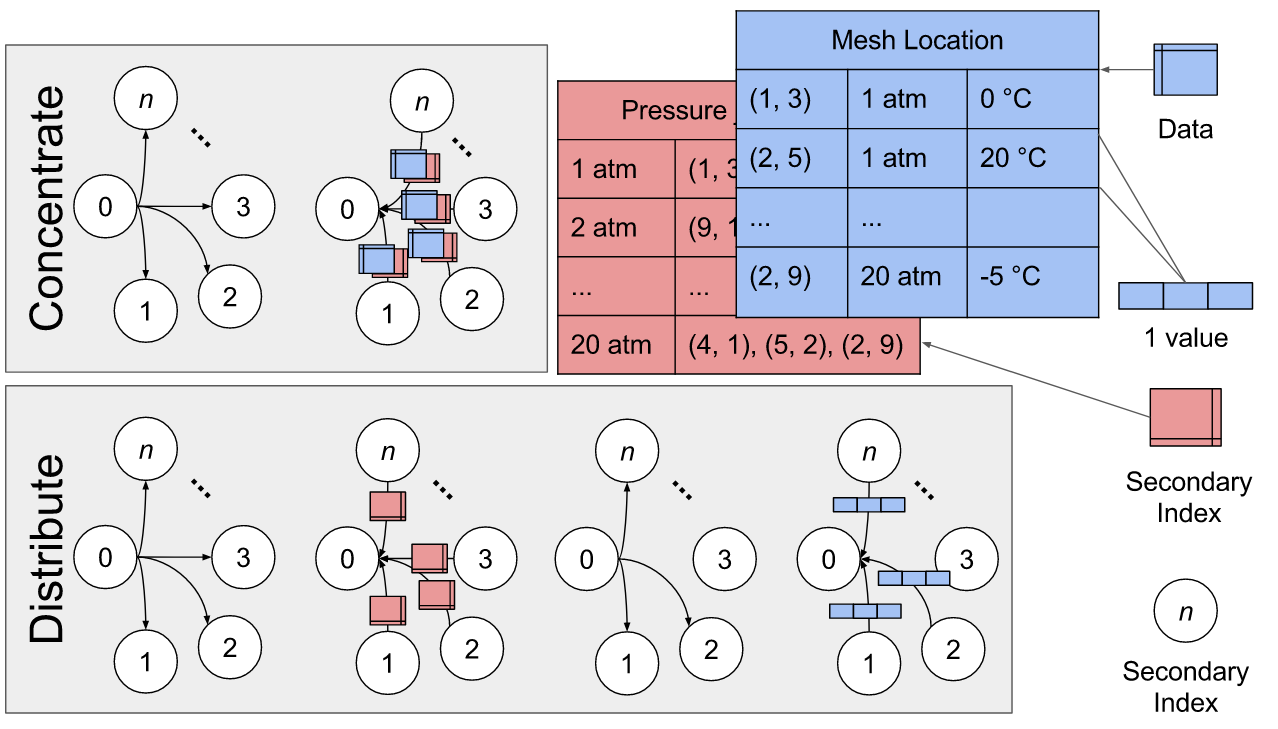
\includegraphics[width=19pc,angle=0]{figures/example.png}\\
  \caption{For a multi-part query with locality, migrating for distribution
  (solution 1) takes more RPCs while migrating for concentration (solution 2)
  risks of overloading the client.}
  \label{fig:example}
\end{figure}

% What is the problem with multipart queries?
Another example is multi-part queries: finding the maximum value \(x\) of the
neighbors in a mesh of another maximum value \(y\).  For example, finding the
highest temperatures of the neighbors of mesh cells with the highest pressure.
Given that the hash is defined by mesh location, finding the highest pressure
is one RPC per server.  Unfortunately, even with an index based on the maximum
pressures, finding the highest temperatures for {\it neighboring} cells with
the highest pressures requires an additional RPC per server. 

% What can the API do?
Specifically, the API helps us explore the space of solutions for these types
of queries. As shown in Figure~\ref{fig:example}, queries with locality have
two solutions: (1) pull the index and re-query every server, or (2) pull the
index and partial set of results that can be satisfied locally. Solution 1
emphasizes distribution and incurrs extra RPCs while Solution 2 opts to
concentrate data at the expense of data transfer, consistency issues, and
increased memory usage.  Both options have advantages but inserting an API to
control the mechanisms helps future programmers quickly evaluate both options
and design solutions for their workload.


